\documentclass[1p]{elsarticle_modified}
%\bibliographystyle{elsarticle-num}

%\usepackage[colorlinks]{hyperref}
%\usepackage{abbrmath_seonhwa} %\Abb, \Ascr, \Acal ,\Abf, \Afrak
\usepackage{amsfonts}
\usepackage{amssymb}
\usepackage{amsmath}
\usepackage{amsthm}
\usepackage{scalefnt}
\usepackage{amsbsy}
\usepackage{kotex}
\usepackage{caption}
\usepackage{subfig}
\usepackage{color}
\usepackage{graphicx}
\usepackage{xcolor} %% white, black, red, green, blue, cyan, magenta, yellow
\usepackage{float}
\usepackage{setspace}
\usepackage{hyperref}

\usepackage{tikz}
\usetikzlibrary{arrows}

\usepackage{multirow}
\usepackage{array} % fixed length table
\usepackage{hhline}

%%%%%%%%%%%%%%%%%%%%%
\makeatletter
\renewcommand*\env@matrix[1][\arraystretch]{%
	\edef\arraystretch{#1}%
	\hskip -\arraycolsep
	\let\@ifnextchar\new@ifnextchar
	\array{*\c@MaxMatrixCols c}}
\makeatother %https://tex.stackexchange.com/questions/14071/how-can-i-increase-the-line-spacing-in-a-matrix
%%%%%%%%%%%%%%%

\usepackage[normalem]{ulem}

\newcommand{\msout}[1]{\ifmmode\text{\sout{\ensuremath{#1}}}\else\sout{#1}\fi}
%SOURCE: \msout is \stkout macro in https://tex.stackexchange.com/questions/20609/strikeout-in-math-mode

\newcommand{\cancel}[1]{
	\ifmmode
	{\color{red}\msout{#1}}
	\else
	{\color{red}\sout{#1}}
	\fi
}

\newcommand{\add}[1]{
	{\color{blue}\uwave{#1}}
}

\newcommand{\replace}[2]{
	\ifmmode
	{\color{red}\msout{#1}}{\color{blue}\uwave{#2}}
	\else
	{\color{red}\sout{#1}}{\color{blue}\uwave{#2}}
	\fi
}

\newcommand{\Sol}{\mathcal{S}} %segment
\newcommand{\D}{D} %diagram
\newcommand{\A}{\mathcal{A}} %arc


%%%%%%%%%%%%%%%%%%%%%%%%%%%%%5 test

\def\sl{\operatorname{\textup{SL}}(2,\Cbb)}
\def\psl{\operatorname{\textup{PSL}}(2,\Cbb)}
\def\quan{\mkern 1mu \triangleright \mkern 1mu}

\theoremstyle{definition}
\newtheorem{thm}{Theorem}[section]
\newtheorem{prop}[thm]{Proposition}
\newtheorem{lem}[thm]{Lemma}
\newtheorem{ques}[thm]{Question}
\newtheorem{cor}[thm]{Corollary}
\newtheorem{defn}[thm]{Definition}
\newtheorem{exam}[thm]{Example}
\newtheorem{rmk}[thm]{Remark}
\newtheorem{alg}[thm]{Algorithm}

\newcommand{\I}{\sqrt{-1}}
\begin{document}

%\begin{frontmatter}
%
%\title{Boundary parabolic representations of knots up to 8 crossings}
%
%%% Group authors per affiliation:
%\author{Yunhi Cho} 
%\address{Department of Mathematics, University of Seoul, Seoul, Korea}
%\ead{yhcho@uos.ac.kr}
%
%
%\author{Seonhwa Kim} %\fnref{s_kim}}
%\address{Center for Geometry and Physics, Institute for Basic Science, Pohang, 37673, Korea}
%\ead{ryeona17@ibs.re.kr}
%
%\author{Hyuk Kim}
%\address{Department of Mathematical Sciences, Seoul National University, Seoul 08826, Korea}
%\ead{hyukkim@snu.ac.kr}
%
%\author{Seokbeom Yoon}
%\address{Department of Mathematical Sciences, Seoul National University, Seoul, 08826,  Korea}
%\ead{sbyoon15@snu.ac.kr}
%
%\begin{abstract}
%We find all boundary parabolic representation of knots up to 8 crossings.
%
%\end{abstract}
%\begin{keyword}
%    \MSC[2010] 57M25 
%\end{keyword}
%
%\end{frontmatter}

%\linenumbers
%\tableofcontents
%
\newcommand\colored[1]{\textcolor{white}{\rule[-0.35ex]{0.8em}{1.4ex}}\kern-0.8em\color{red} #1}%
%\newcommand\colored[1]{\textcolor{white}{ #1}\kern-2.17ex	\textcolor{white}{ #1}\kern-1.81ex	\textcolor{white}{ #1}\kern-2.15ex\color{red}#1	}

{\Large $\underline{12a_{0824}~(K12a_{0824})}$}

\setlength{\tabcolsep}{10pt}
\renewcommand{\arraystretch}{1.6}
\vspace{1cm}\begin{tabular}{m{100pt}>{\centering\arraybackslash}m{274pt}}
\multirow{5}{120pt}{
	\centering
	\includegraphics[width=112pt]{../../../GIT/diagram.site/Diagrams/png/1625_12a_0824.png}\\
\ \ \ A knot diagram\footnotemark}&
\allowdisplaybreaks
\textbf{Linearized knot diagam} \\
\cline{2-2}
 &
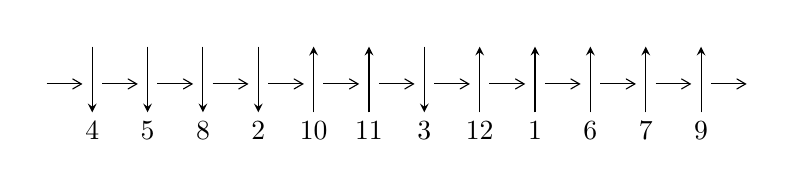
\begin{tikzpicture}[x=20pt, y=17pt]
	% nodes
	\node (C0) at (0, 0) {};
	\node (C1) at (1, 0) {};
	\node (C1U) at (1, +1) {};
	\node (C1D) at (1, -1) {4};

	\node (C2) at (2, 0) {};
	\node (C2U) at (2, +1) {};
	\node (C2D) at (2, -1) {5};

	\node (C3) at (3, 0) {};
	\node (C3U) at (3, +1) {};
	\node (C3D) at (3, -1) {8};

	\node (C4) at (4, 0) {};
	\node (C4U) at (4, +1) {};
	\node (C4D) at (4, -1) {2};

	\node (C5) at (5, 0) {};
	\node (C5U) at (5, +1) {};
	\node (C5D) at (5, -1) {10};

	\node (C6) at (6, 0) {};
	\node (C6U) at (6, +1) {};
	\node (C6D) at (6, -1) {11};

	\node (C7) at (7, 0) {};
	\node (C7U) at (7, +1) {};
	\node (C7D) at (7, -1) {3};

	\node (C8) at (8, 0) {};
	\node (C8U) at (8, +1) {};
	\node (C8D) at (8, -1) {12};

	\node (C9) at (9, 0) {};
	\node (C9U) at (9, +1) {};
	\node (C9D) at (9, -1) {1};

	\node (C10) at (10, 0) {};
	\node (C10U) at (10, +1) {};
	\node (C10D) at (10, -1) {6};

	\node (C11) at (11, 0) {};
	\node (C11U) at (11, +1) {};
	\node (C11D) at (11, -1) {7};

	\node (C12) at (12, 0) {};
	\node (C12U) at (12, +1) {};
	\node (C12D) at (12, -1) {9};
	\node (C13) at (13, 0) {};

	% arrows
	\draw[->,>={angle 60}]
	(C0) edge (C1) (C1) edge (C2) (C2) edge (C3) (C3) edge (C4) (C4) edge (C5) (C5) edge (C6) (C6) edge (C7) (C7) edge (C8) (C8) edge (C9) (C9) edge (C10) (C10) edge (C11) (C11) edge (C12) (C12) edge (C13) ;	\draw[->,>=stealth]
	(C1U) edge (C1D) (C2U) edge (C2D) (C3U) edge (C3D) (C4U) edge (C4D) (C5D) edge (C5U) (C6D) edge (C6U) (C7U) edge (C7D) (C8D) edge (C8U) (C9D) edge (C9U) (C10D) edge (C10U) (C11D) edge (C11U) (C12D) edge (C12U) ;
	\end{tikzpicture} \\
\hhline{~~} \\& 
\textbf{Solving Sequence} \\ \cline{2-2} 
 &
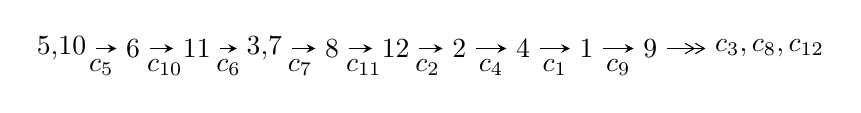
\begin{tikzpicture}[x=23pt, y=7pt]
	% node
	\node (A0) at (-1/8, 0) {5,10};
	\node (A1) at (1, 0) {6};
	\node (A2) at (2, 0) {11};
	\node (A3) at (49/16, 0) {3,7};
	\node (A4) at (33/8, 0) {8};
	\node (A5) at (41/8, 0) {12};
	\node (A6) at (49/8, 0) {2};
	\node (A7) at (57/8, 0) {4};
	\node (A8) at (65/8, 0) {1};
	\node (A9) at (73/8, 0) {9};
	\node (C1) at (1/2, -1) {$c_{5}$};
	\node (C2) at (3/2, -1) {$c_{10}$};
	\node (C3) at (5/2, -1) {$c_{6}$};
	\node (C4) at (29/8, -1) {$c_{7}$};
	\node (C5) at (37/8, -1) {$c_{11}$};
	\node (C6) at (45/8, -1) {$c_{2}$};
	\node (C7) at (53/8, -1) {$c_{4}$};
	\node (C8) at (61/8, -1) {$c_{1}$};
	\node (C9) at (69/8, -1) {$c_{9}$};
	\node (A10) at (11, 0) {$c_{3},c_{8},c_{12}$};

	% edge
	\draw[->,>=stealth]	
	(A0) edge (A1) (A1) edge (A2) (A2) edge (A3) (A3) edge (A4) (A4) edge (A5) (A5) edge (A6) (A6) edge (A7) (A7) edge (A8) (A8) edge (A9) ;
	\draw[->>,>={angle 60}]	
	(A9) edge (A10);
\end{tikzpicture} \\ 

\end{tabular} \\

\footnotetext{
The image of knot diagram is generated by the software ``\textbf{Draw programme}" developed by Andrew Bartholomew(\url{http://www.layer8.co.uk/maths/draw/index.htm\#Running-draw}), where we modified some parts for our purpose(\url{https://github.com/CATsTAILs/LinksPainter}).
}\phantom \\ \newline 
\centering \textbf{Ideals for irreducible components\footnotemark of $X_{\text{par}}$} 
 
\begin{align*}
I^u_{1}&=\langle 
2.98047\times10^{56} u^{61}-7.28716\times10^{56} u^{60}+\cdots+2.15534\times10^{55} b-3.50669\times10^{57},\\
\phantom{I^u_{1}}&\phantom{= \langle  }-3.70578\times10^{56} u^{61}+9.04815\times10^{56} u^{60}+\cdots+2.15534\times10^{55} a+4.10393\times10^{57},\\
\phantom{I^u_{1}}&\phantom{= \langle  }u^{62}-2 u^{61}+\cdots-12 u-4\rangle \\
I^u_{2}&=\langle 
b+1,\;u^2+a+u-2,\;u^3+u^2-2 u-1\rangle \\
I^u_{3}&=\langle 
a u+b+2 a-1,\;2 a^2+a u-2 a+2 u-3,\;u^2-2\rangle \\
\\
I^v_{1}&=\langle 
a,\;b+v-2,\;v^2-3 v+1\rangle \\
\end{align*}
\raggedright * 4 irreducible components of $\dim_{\mathbb{C}}=0$, with total 71 representations.\\
\footnotetext{All coefficients of polynomials are rational numbers. But the coefficients are sometimes approximated in decimal forms when there is not enough margin.}
\newpage
\renewcommand{\arraystretch}{1}
\centering \section*{I. $I^u_{1}= \langle 2.98\times10^{56} u^{61}-7.29\times10^{56} u^{60}+\cdots+2.16\times10^{55} b-3.51\times10^{57},\;-3.71\times10^{56} u^{61}+9.05\times10^{56} u^{60}+\cdots+2.16\times10^{55} a+4.10\times10^{57},\;u^{62}-2 u^{61}+\cdots-12 u-4 \rangle$}
\flushleft \textbf{(i) Arc colorings}\\
\begin{tabular}{m{7pt} m{180pt} m{7pt} m{180pt} }
\flushright $a_{5}=$&$\begin{pmatrix}1\\0\end{pmatrix}$ \\
\flushright $a_{10}=$&$\begin{pmatrix}0\\u\end{pmatrix}$ \\
\flushright $a_{6}=$&$\begin{pmatrix}1\\- u^2\end{pmatrix}$ \\
\flushright $a_{11}=$&$\begin{pmatrix}u\\- u^3+u\end{pmatrix}$ \\
\flushright $a_{3}=$&$\begin{pmatrix}17.1935 u^{61}-41.9802 u^{60}+\cdots-59.0803 u-190.408\\-13.8283 u^{61}+33.8098 u^{60}+\cdots+35.7338 u+162.698\end{pmatrix}$ \\
\flushright $a_{7}=$&$\begin{pmatrix}- u^2+1\\u^4-2 u^2\end{pmatrix}$ \\
\flushright $a_{8}=$&$\begin{pmatrix}1.21636 u^{61}-2.59080 u^{60}+\cdots-18.6035 u-0.834246\\-22.4729 u^{61}+50.9927 u^{60}+\cdots+34.3595 u+239.437\end{pmatrix}$ \\
\flushright $a_{12}=$&$\begin{pmatrix}- u^3+2 u\\u^5-3 u^3+u\end{pmatrix}$ \\
\flushright $a_{2}=$&$\begin{pmatrix}3.36518 u^{61}-8.17039 u^{60}+\cdots-23.3465 u-27.7096\\-13.8283 u^{61}+33.8098 u^{60}+\cdots+35.7338 u+162.698\end{pmatrix}$ \\
\flushright $a_{4}=$&$\begin{pmatrix}38.7754 u^{61}-92.5739 u^{60}+\cdots-86.8745 u-442.022\\17.6227 u^{61}-43.4791 u^{60}+\cdots-45.7098 u-215.395\end{pmatrix}$ \\
\flushright $a_{1}=$&$\begin{pmatrix}39.6334 u^{61}-94.3136 u^{60}+\cdots-95.8498 u-449.301\\17.1297 u^{61}-42.0208 u^{60}+\cdots-39.9181 u-209.663\end{pmatrix}$ \\
\flushright $a_{9}=$&$\begin{pmatrix}-8.92692 u^{61}+20.4057 u^{60}+\cdots-0.725611 u+105.357\\-26.0460 u^{61}+58.7518 u^{60}+\cdots+38.2629 u+274.601\end{pmatrix}$\\&\end{tabular}
\flushleft \textbf{(ii) Obstruction class $= -1$}\\~\\
\flushleft \textbf{(iii) Cusp Shapes $= -2.64973 u^{61}+4.67865 u^{60}+\cdots-82.0084 u+32.7971$}\\~\\
\newpage\renewcommand{\arraystretch}{1}
\flushleft \textbf{(iv) u-Polynomials at the component}\newline \\
\begin{tabular}{m{50pt}|m{274pt}}
Crossings & \hspace{64pt}u-Polynomials at each crossing \\
\hline $$\begin{aligned}c_{1},c_{2},c_{4}\end{aligned}$$&$\begin{aligned}
&u^{62}-7 u^{61}+\cdots+29 u+1
\end{aligned}$\\
\hline $$\begin{aligned}c_{3},c_{7}\end{aligned}$$&$\begin{aligned}
&u^{62}-2 u^{61}+\cdots+108 u-8
\end{aligned}$\\
\hline $$\begin{aligned}c_{5},c_{6},c_{10}\\c_{11}\end{aligned}$$&$\begin{aligned}
&u^{62}+2 u^{61}+\cdots+12 u-4
\end{aligned}$\\
\hline $$\begin{aligned}c_{8},c_{9},c_{12}\end{aligned}$$&$\begin{aligned}
&u^{62}-4 u^{61}+\cdots+81 u-9
\end{aligned}$\\
\hline
\end{tabular}\\~\\
\newpage\renewcommand{\arraystretch}{1}
\flushleft \textbf{(v) Riley Polynomials at the component}\newline \\
\begin{tabular}{m{50pt}|m{274pt}}
Crossings & \hspace{64pt}Riley Polynomials at each crossing \\
\hline $$\begin{aligned}c_{1},c_{2},c_{4}\end{aligned}$$&$\begin{aligned}
&y^{62}-57 y^{61}+\cdots-427 y+1
\end{aligned}$\\
\hline $$\begin{aligned}c_{3},c_{7}\end{aligned}$$&$\begin{aligned}
&y^{62}-30 y^{61}+\cdots-4688 y+64
\end{aligned}$\\
\hline $$\begin{aligned}c_{5},c_{6},c_{10}\\c_{11}\end{aligned}$$&$\begin{aligned}
&y^{62}-74 y^{61}+\cdots-624 y+16
\end{aligned}$\\
\hline $$\begin{aligned}c_{8},c_{9},c_{12}\end{aligned}$$&$\begin{aligned}
&y^{62}-60 y^{61}+\cdots-3519 y+81
\end{aligned}$\\
\hline
\end{tabular}\\~\\
\newpage\flushleft \textbf{(vi) Complex Volumes and Cusp Shapes}
$$\begin{array}{c|c|c}  
\text{Solutions to }I^u_{1}& \I (\text{vol} + \sqrt{-1}CS) & \text{Cusp shape}\\
 \hline 
\begin{aligned}
u &= -0.728927 + 0.693480 I \\
a &= \phantom{-}0.50031 - 1.40841 I \\
b &= \phantom{-}1.41056 + 0.37112 I\end{aligned}
 & -0.16183 - 11.03280 I & \phantom{-0.000000 } 0 \\ \hline\begin{aligned}
u &= -0.728927 - 0.693480 I \\
a &= \phantom{-}0.50031 + 1.40841 I \\
b &= \phantom{-}1.41056 - 0.37112 I\end{aligned}
 & -0.16183 + 11.03280 I & \phantom{-0.000000 } 0 \\ \hline\begin{aligned}
u &= \phantom{-}0.979023 + 0.319186 I \\
a &= \phantom{-}0.687788 + 0.612198 I \\
b &= \phantom{-}0.174252 - 0.593165 I\end{aligned}
 & \phantom{-}6.85692 + 1.08905 I & \phantom{-0.000000 } 0 \\ \hline\begin{aligned}
u &= \phantom{-}0.979023 - 0.319186 I \\
a &= \phantom{-}0.687788 - 0.612198 I \\
b &= \phantom{-}0.174252 + 0.593165 I\end{aligned}
 & \phantom{-}6.85692 - 1.08905 I & \phantom{-0.000000 } 0 \\ \hline\begin{aligned}
u &= -0.869463 + 0.382228 I \\
a &= -0.78515 - 1.20030 I \\
b &= \phantom{-}1.394320 + 0.085865 I\end{aligned}
 & -4.30575 - 1.13280 I & \phantom{-0.000000 } 0 \\ \hline\begin{aligned}
u &= -0.869463 - 0.382228 I \\
a &= -0.78515 + 1.20030 I \\
b &= \phantom{-}1.394320 - 0.085865 I\end{aligned}
 & -4.30575 + 1.13280 I & \phantom{-0.000000 } 0 \\ \hline\begin{aligned}
u &= \phantom{-}0.744058 + 0.573909 I \\
a &= \phantom{-}0.05054 + 1.60912 I \\
b &= \phantom{-}1.41065 - 0.23730 I\end{aligned}
 & -5.93385 + 6.46887 I & \phantom{-0.000000 } 0. - 6.93804 I \\ \hline\begin{aligned}
u &= \phantom{-}0.744058 - 0.573909 I \\
a &= \phantom{-}0.05054 - 1.60912 I \\
b &= \phantom{-}1.41065 + 0.23730 I\end{aligned}
 & -5.93385 - 6.46887 I & \phantom{-0.000000 -}0. + 6.93804 I \\ \hline\begin{aligned}
u &= -0.757731 + 0.545713 I \\
a &= -0.418942 + 0.852081 I \\
b &= -0.234673 - 0.886336 I\end{aligned}
 & \phantom{-}5.04847 - 6.51467 I & \phantom{-0.000000 -}0. + 6.90536 I \\ \hline\begin{aligned}
u &= -0.757731 - 0.545713 I \\
a &= -0.418942 - 0.852081 I \\
b &= -0.234673 + 0.886336 I\end{aligned}
 & \phantom{-}5.04847 + 6.51467 I & \phantom{-0.000000 } 0. - 6.90536 I\\
 \hline 
 \end{array}$$\newpage$$\begin{array}{c|c|c}  
\text{Solutions to }I^u_{1}& \I (\text{vol} + \sqrt{-1}CS) & \text{Cusp shape}\\
 \hline 
\begin{aligned}
u &= -0.294207 + 0.839087 I \\
a &= \phantom{-}0.678495 - 0.208859 I \\
b &= \phantom{-}1.351380 - 0.291230 I\end{aligned}
 & -1.47807 + 5.97196 I & \phantom{-}0.82075 - 3.88105 I \\ \hline\begin{aligned}
u &= -0.294207 - 0.839087 I \\
a &= \phantom{-}0.678495 + 0.208859 I \\
b &= \phantom{-}1.351380 + 0.291230 I\end{aligned}
 & -1.47807 - 5.97196 I & \phantom{-}0.82075 + 3.88105 I \\ \hline\begin{aligned}
u &= \phantom{-}0.700864 + 0.454130 I \\
a &= -1.08574 - 1.35076 I \\
b &= -1.381210 + 0.269324 I\end{aligned}
 & \phantom{-}1.85807 + 4.31924 I & \phantom{-}4.65831 - 4.87668 I \\ \hline\begin{aligned}
u &= \phantom{-}0.700864 - 0.454130 I \\
a &= -1.08574 + 1.35076 I \\
b &= -1.381210 - 0.269324 I\end{aligned}
 & \phantom{-}1.85807 - 4.31924 I & \phantom{-}4.65831 + 4.87668 I \\ \hline\begin{aligned}
u &= -0.720139 + 0.323549 I \\
a &= -0.041734 - 0.370738 I \\
b &= -0.990063 + 0.574650 I\end{aligned}
 & \phantom{-}2.74398 - 1.42912 I & \phantom{-}4.95658 + 3.06315 I \\ \hline\begin{aligned}
u &= -0.720139 - 0.323549 I \\
a &= -0.041734 + 0.370738 I \\
b &= -0.990063 - 0.574650 I\end{aligned}
 & \phantom{-}2.74398 + 1.42912 I & \phantom{-}4.95658 - 3.06315 I \\ \hline\begin{aligned}
u &= \phantom{-}0.612514 + 0.397650 I \\
a &= -0.270980 - 1.353370 I \\
b &= -0.326776 + 0.647435 I\end{aligned}
 & -0.38950 + 3.27691 I & \phantom{-}2.40587 - 8.31237 I \\ \hline\begin{aligned}
u &= \phantom{-}0.612514 - 0.397650 I \\
a &= -0.270980 + 1.353370 I \\
b &= -0.326776 - 0.647435 I\end{aligned}
 & -0.38950 - 3.27691 I & \phantom{-}2.40587 + 8.31237 I \\ \hline\begin{aligned}
u &= -0.154333 + 0.690721 I \\
a &= \phantom{-}0.498196 + 0.076734 I \\
b &= -0.141589 + 0.700436 I\end{aligned}
 & \phantom{-}3.24167 + 2.36306 I & \phantom{-}4.92638 - 2.57172 I \\ \hline\begin{aligned}
u &= -0.154333 - 0.690721 I \\
a &= \phantom{-}0.498196 - 0.076734 I \\
b &= -0.141589 - 0.700436 I\end{aligned}
 & \phantom{-}3.24167 - 2.36306 I & \phantom{-}4.92638 + 2.57172 I\\
 \hline 
 \end{array}$$\newpage$$\begin{array}{c|c|c}  
\text{Solutions to }I^u_{1}& \I (\text{vol} + \sqrt{-1}CS) & \text{Cusp shape}\\
 \hline 
\begin{aligned}
u &= \phantom{-}0.168802 + 0.683958 I \\
a &= \phantom{-}0.772109 + 0.104136 I \\
b &= \phantom{-}1.43972 + 0.11421 I\end{aligned}
 & -7.63058 - 2.23574 I & -4.95663 + 1.98264 I \\ \hline\begin{aligned}
u &= \phantom{-}0.168802 - 0.683958 I \\
a &= \phantom{-}0.772109 - 0.104136 I \\
b &= \phantom{-}1.43972 - 0.11421 I\end{aligned}
 & -7.63058 + 2.23574 I & -4.95663 - 1.98264 I \\ \hline\begin{aligned}
u &= -1.35461\phantom{ +0.000000I} \\
a &= -0.662234\phantom{ +0.000000I} \\
b &= \phantom{-}1.56599\phantom{ +0.000000I}\end{aligned}
 & -3.74962\phantom{ +0.000000I} & \phantom{-0.000000 } 0 \\ \hline\begin{aligned}
u &= -0.472149 + 0.408625 I \\
a &= -1.37617 + 1.82546 I \\
b &= -1.274780 - 0.089703 I\end{aligned}
 & -2.79224 - 1.47778 I & -0.57816 + 4.38549 I \\ \hline\begin{aligned}
u &= -0.472149 - 0.408625 I \\
a &= -1.37617 - 1.82546 I \\
b &= -1.274780 + 0.089703 I\end{aligned}
 & -2.79224 + 1.47778 I & -0.57816 - 4.38549 I \\ \hline\begin{aligned}
u &= \phantom{-}1.37684\phantom{ +0.000000I} \\
a &= \phantom{-}0.886850\phantom{ +0.000000I} \\
b &= -0.0476686\phantom{ +0.000000I}\end{aligned}
 & \phantom{-}6.50761\phantom{ +0.000000I} & \phantom{-0.000000 } 0 \\ \hline\begin{aligned}
u &= \phantom{-}1.315790 + 0.425847 I \\
a &= -0.397092 + 0.322882 I \\
b &= \phantom{-}1.255370 + 0.180857 I\end{aligned}
 & \phantom{-}3.54224 - 1.50691 I & \phantom{-0.000000 } 0 \\ \hline\begin{aligned}
u &= \phantom{-}1.315790 - 0.425847 I \\
a &= -0.397092 - 0.322882 I \\
b &= \phantom{-}1.255370 - 0.180857 I\end{aligned}
 & \phantom{-}3.54224 + 1.50691 I & \phantom{-0.000000 } 0 \\ \hline\begin{aligned}
u &= -1.43056\phantom{ +0.000000I} \\
a &= \phantom{-}8.65850\phantom{ +0.000000I} \\
b &= -0.979198\phantom{ +0.000000I}\end{aligned}
 & \phantom{-}4.96917\phantom{ +0.000000I} & \phantom{-0.000000 } 0 \\ \hline\begin{aligned}
u &= \phantom{-}0.150519 + 0.505903 I \\
a &= -3.05850 - 1.07646 I \\
b &= -1.166570 - 0.207757 I\end{aligned}
 & \phantom{-}0.273379 - 0.971704 I & \phantom{-}0.08959 - 3.04439 I\\
 \hline 
 \end{array}$$\newpage$$\begin{array}{c|c|c}  
\text{Solutions to }I^u_{1}& \I (\text{vol} + \sqrt{-1}CS) & \text{Cusp shape}\\
 \hline 
\begin{aligned}
u &= \phantom{-}0.150519 - 0.505903 I \\
a &= -3.05850 + 1.07646 I \\
b &= -1.166570 + 0.207757 I\end{aligned}
 & \phantom{-}0.273379 + 0.971704 I & \phantom{-}0.08959 + 3.04439 I \\ \hline\begin{aligned}
u &= -0.523123 + 0.028134 I \\
a &= \phantom{-}1.13938 - 0.89193 I \\
b &= -0.084530 + 0.244571 I\end{aligned}
 & \phantom{-}0.906568 - 0.098785 I & \phantom{-}10.73700 + 0.03939 I \\ \hline\begin{aligned}
u &= -0.523123 - 0.028134 I \\
a &= \phantom{-}1.13938 + 0.89193 I \\
b &= -0.084530 - 0.244571 I\end{aligned}
 & \phantom{-}0.906568 + 0.098785 I & \phantom{-}10.73700 - 0.03939 I \\ \hline\begin{aligned}
u &= -1.51079 + 0.03677 I \\
a &= \phantom{-}1.03861 - 1.20593 I \\
b &= -0.962369 + 0.432397 I\end{aligned}
 & \phantom{-}4.73047 - 0.55582 I & \phantom{-0.000000 } 0 \\ \hline\begin{aligned}
u &= -1.51079 - 0.03677 I \\
a &= \phantom{-}1.03861 + 1.20593 I \\
b &= -0.962369 - 0.432397 I\end{aligned}
 & \phantom{-}4.73047 + 0.55582 I & \phantom{-0.000000 } 0 \\ \hline\begin{aligned}
u &= \phantom{-}0.280851 + 0.380725 I \\
a &= \phantom{-}0.583491 + 0.202281 I \\
b &= -0.543197 - 0.407436 I\end{aligned}
 & -1.335370 - 0.411278 I & -3.93368 + 0.07785 I \\ \hline\begin{aligned}
u &= \phantom{-}0.280851 - 0.380725 I \\
a &= \phantom{-}0.583491 - 0.202281 I \\
b &= -0.543197 + 0.407436 I\end{aligned}
 & -1.335370 + 0.411278 I & -3.93368 - 0.07785 I \\ \hline\begin{aligned}
u &= \phantom{-}1.53718 + 0.08815 I \\
a &= \phantom{-}0.26347 - 1.53965 I \\
b &= -1.318230 + 0.251318 I\end{aligned}
 & \phantom{-}3.97848 + 3.12179 I & \phantom{-0.000000 } 0 \\ \hline\begin{aligned}
u &= \phantom{-}1.53718 - 0.08815 I \\
a &= \phantom{-}0.26347 + 1.53965 I \\
b &= -1.318230 - 0.251318 I\end{aligned}
 & \phantom{-}3.97848 - 3.12179 I & \phantom{-0.000000 } 0 \\ \hline\begin{aligned}
u &= \phantom{-}1.54676\phantom{ +0.000000I} \\
a &= -0.552532\phantom{ +0.000000I} \\
b &= \phantom{-}1.77372\phantom{ +0.000000I}\end{aligned}
 & -0.257952\phantom{ +0.000000I} & \phantom{-0.000000 } 0\\
 \hline 
 \end{array}$$\newpage$$\begin{array}{c|c|c}  
\text{Solutions to }I^u_{1}& \I (\text{vol} + \sqrt{-1}CS) & \text{Cusp shape}\\
 \hline 
\begin{aligned}
u &= \phantom{-}1.58047 + 0.01988 I \\
a &= \phantom{-}0.307453 - 1.365900 I \\
b &= \phantom{-}0.028298 + 0.630886 I\end{aligned}
 & \phantom{-}8.23798 + 0.05802 I & \phantom{-0.000000 } 0 \\ \hline\begin{aligned}
u &= \phantom{-}1.58047 - 0.01988 I \\
a &= \phantom{-}0.307453 + 1.365900 I \\
b &= \phantom{-}0.028298 - 0.630886 I\end{aligned}
 & \phantom{-}8.23798 - 0.05802 I & \phantom{-0.000000 } 0 \\ \hline\begin{aligned}
u &= -1.58423 + 0.10551 I \\
a &= \phantom{-}0.00098 + 1.59403 I \\
b &= -0.206251 - 0.827340 I\end{aligned}
 & \phantom{-}7.10069 - 5.07913 I & \phantom{-0.000000 } 0 \\ \hline\begin{aligned}
u &= -1.58423 - 0.10551 I \\
a &= \phantom{-}0.00098 - 1.59403 I \\
b &= -0.206251 + 0.827340 I\end{aligned}
 & \phantom{-}7.10069 + 5.07913 I & \phantom{-0.000000 } 0 \\ \hline\begin{aligned}
u &= -1.60674 + 0.13048 I \\
a &= \phantom{-}0.203247 + 1.201000 I \\
b &= -1.51444 - 0.32292 I\end{aligned}
 & \phantom{-}9.71439 - 6.49643 I & \phantom{-0.000000 } 0 \\ \hline\begin{aligned}
u &= -1.60674 - 0.13048 I \\
a &= \phantom{-}0.203247 - 1.201000 I \\
b &= -1.51444 + 0.32292 I\end{aligned}
 & \phantom{-}9.71439 + 6.49643 I & \phantom{-0.000000 } 0 \\ \hline\begin{aligned}
u &= \phantom{-}1.61104 + 0.09528 I \\
a &= \phantom{-}0.709620 + 0.974902 I \\
b &= -1.082630 - 0.771501 I\end{aligned}
 & \phantom{-}10.73290 + 3.02061 I & \phantom{-0.000000 } 0 \\ \hline\begin{aligned}
u &= \phantom{-}1.61104 - 0.09528 I \\
a &= \phantom{-}0.709620 - 0.974902 I \\
b &= -1.082630 + 0.771501 I\end{aligned}
 & \phantom{-}10.73290 - 3.02061 I & \phantom{-0.000000 } 0 \\ \hline\begin{aligned}
u &= -1.61936 + 0.17707 I \\
a &= -0.71301 - 1.47528 I \\
b &= \phantom{-}1.38942 + 0.34866 I\end{aligned}
 & \phantom{-}2.05187 - 9.32176 I & \phantom{-0.000000 } 0 \\ \hline\begin{aligned}
u &= -1.61936 - 0.17707 I \\
a &= -0.71301 + 1.47528 I \\
b &= \phantom{-}1.38942 - 0.34866 I\end{aligned}
 & \phantom{-}2.05187 + 9.32176 I & \phantom{-0.000000 } 0\\
 \hline 
 \end{array}$$\newpage$$\begin{array}{c|c|c}  
\text{Solutions to }I^u_{1}& \I (\text{vol} + \sqrt{-1}CS) & \text{Cusp shape}\\
 \hline 
\begin{aligned}
u &= \phantom{-}1.62558 + 0.16107 I \\
a &= -0.18148 - 1.48352 I \\
b &= -0.265871 + 1.040180 I\end{aligned}
 & \phantom{-}13.1382 + 9.1870 I & \phantom{-0.000000 } 0 \\ \hline\begin{aligned}
u &= \phantom{-}1.62558 - 0.16107 I \\
a &= -0.18148 + 1.48352 I \\
b &= -0.265871 - 1.040180 I\end{aligned}
 & \phantom{-}13.1382 - 9.1870 I & \phantom{-0.000000 } 0 \\ \hline\begin{aligned}
u &= \phantom{-}1.61953 + 0.21948 I \\
a &= -0.42080 + 1.54749 I \\
b &= \phantom{-}1.45736 - 0.44242 I\end{aligned}
 & \phantom{-}7.6958 + 14.4824 I & \phantom{-0.000000 } 0 \\ \hline\begin{aligned}
u &= \phantom{-}1.61953 - 0.21948 I \\
a &= -0.42080 - 1.54749 I \\
b &= \phantom{-}1.45736 + 0.44242 I\end{aligned}
 & \phantom{-}7.6958 - 14.4824 I & \phantom{-0.000000 } 0 \\ \hline\begin{aligned}
u &= -0.363008\phantom{ +0.000000I} \\
a &= \phantom{-}3.16745\phantom{ +0.000000I} \\
b &= -0.297973\phantom{ +0.000000I}\end{aligned}
 & \phantom{-}0.945431\phantom{ +0.000000I} & \phantom{-}16.1240\phantom{ +0.000000I} \\ \hline\begin{aligned}
u &= -0.353073\phantom{ +0.000000I} \\
a &= \phantom{-}1.07459\phantom{ +0.000000I} \\
b &= \phantom{-}1.65773\phantom{ +0.000000I}\end{aligned}
 & -6.97573\phantom{ +0.000000I} & \phantom{-}16.8660\phantom{ +0.000000I} \\ \hline\begin{aligned}
u &= \phantom{-}1.65034 + 0.12971 I \\
a &= -0.97563 + 1.03708 I \\
b &= \phantom{-}1.278460 - 0.240889 I\end{aligned}
 & \phantom{-}4.33770 + 3.20222 I & \phantom{-0.000000 } 0 \\ \hline\begin{aligned}
u &= \phantom{-}1.65034 - 0.12971 I \\
a &= -0.97563 - 1.03708 I \\
b &= \phantom{-}1.278460 + 0.240889 I\end{aligned}
 & \phantom{-}4.33770 - 3.20222 I & \phantom{-0.000000 } 0 \\ \hline\begin{aligned}
u &= -1.67507 + 0.05882 I \\
a &= \phantom{-}0.039583 - 1.084640 I \\
b &= \phantom{-}0.468851 + 0.766491 I\end{aligned}
 & \phantom{-}16.0964 - 2.4237 I & \phantom{-0.000000 } 0 \\ \hline\begin{aligned}
u &= -1.67507 - 0.05882 I \\
a &= \phantom{-}0.039583 + 1.084640 I \\
b &= \phantom{-}0.468851 - 0.766491 I\end{aligned}
 & \phantom{-}16.0964 + 2.4237 I & \phantom{-0.000000 } 0\\
 \hline 
 \end{array}$$\newpage$$\begin{array}{c|c|c}  
\text{Solutions to }I^u_{1}& \I (\text{vol} + \sqrt{-1}CS) & \text{Cusp shape}\\
 \hline 
\begin{aligned}
u &= \phantom{-}0.284099\phantom{ +0.000000I} \\
a &= \phantom{-}2.60629\phantom{ +0.000000I} \\
b &= -0.896150\phantom{ +0.000000I}\end{aligned}
 & -1.25065\phantom{ +0.000000I} & -13.1380\phantom{ +0.000000I} \\ \hline\begin{aligned}
u &= -1.82703\phantom{ +0.000000I} \\
a &= -0.674961\phantom{ +0.000000I} \\
b &= \phantom{-}1.09260\phantom{ +0.000000I}\end{aligned}
 & \phantom{-}15.7512\phantom{ +0.000000I} & \phantom{-0.000000 } 0\\
 \hline 
 \end{array}$$\newpage\newpage\renewcommand{\arraystretch}{1}
\centering \section*{II. $I^u_{2}= \langle b+1,\;u^2+a+u-2,\;u^3+u^2-2 u-1 \rangle$}
\flushleft \textbf{(i) Arc colorings}\\
\begin{tabular}{m{7pt} m{180pt} m{7pt} m{180pt} }
\flushright $a_{5}=$&$\begin{pmatrix}1\\0\end{pmatrix}$ \\
\flushright $a_{10}=$&$\begin{pmatrix}0\\u\end{pmatrix}$ \\
\flushright $a_{6}=$&$\begin{pmatrix}1\\- u^2\end{pmatrix}$ \\
\flushright $a_{11}=$&$\begin{pmatrix}u\\u^2- u-1\end{pmatrix}$ \\
\flushright $a_{3}=$&$\begin{pmatrix}- u^2- u+2\\-1\end{pmatrix}$ \\
\flushright $a_{7}=$&$\begin{pmatrix}- u^2+1\\u^2- u-1\end{pmatrix}$ \\
\flushright $a_{8}=$&$\begin{pmatrix}- u^2+1\\u^2- u-1\end{pmatrix}$ \\
\flushright $a_{12}=$&$\begin{pmatrix}u^2-1\\- u^2\end{pmatrix}$ \\
\flushright $a_{2}=$&$\begin{pmatrix}- u^2- u+1\\-1\end{pmatrix}$ \\
\flushright $a_{4}=$&$\begin{pmatrix}- u^2- u+2\\-1\end{pmatrix}$ \\
\flushright $a_{1}=$&$\begin{pmatrix}-1\\0\end{pmatrix}$ \\
\flushright $a_{9}=$&$\begin{pmatrix}- u\\u\end{pmatrix}$\\&\end{tabular}
\flushleft \textbf{(ii) Obstruction class $= 1$}\\~\\
\flushleft \textbf{(iii) Cusp Shapes $= u^2-4 u+12$}\\~\\
\newpage\renewcommand{\arraystretch}{1}
\flushleft \textbf{(iv) u-Polynomials at the component}\newline \\
\begin{tabular}{m{50pt}|m{274pt}}
Crossings & \hspace{64pt}u-Polynomials at each crossing \\
\hline $$\begin{aligned}c_{1},c_{2}\end{aligned}$$&$\begin{aligned}
&(u-1)^3
\end{aligned}$\\
\hline $$\begin{aligned}c_{3},c_{7}\end{aligned}$$&$\begin{aligned}
&u^3
\end{aligned}$\\
\hline $$\begin{aligned}c_{4}\end{aligned}$$&$\begin{aligned}
&(u+1)^3
\end{aligned}$\\
\hline $$\begin{aligned}c_{5},c_{6},c_{8}\\c_{9}\end{aligned}$$&$\begin{aligned}
&u^3+u^2-2 u-1
\end{aligned}$\\
\hline $$\begin{aligned}c_{10},c_{11},c_{12}\end{aligned}$$&$\begin{aligned}
&u^3- u^2-2 u+1
\end{aligned}$\\
\hline
\end{tabular}\\~\\
\newpage\renewcommand{\arraystretch}{1}
\flushleft \textbf{(v) Riley Polynomials at the component}\newline \\
\begin{tabular}{m{50pt}|m{274pt}}
Crossings & \hspace{64pt}Riley Polynomials at each crossing \\
\hline $$\begin{aligned}c_{1},c_{2},c_{4}\end{aligned}$$&$\begin{aligned}
&(y-1)^3
\end{aligned}$\\
\hline $$\begin{aligned}c_{3},c_{7}\end{aligned}$$&$\begin{aligned}
&y^3
\end{aligned}$\\
\hline $$\begin{aligned}c_{5},c_{6},c_{8}\\c_{9},c_{10},c_{11}\\c_{12}\end{aligned}$$&$\begin{aligned}
&y^3-5 y^2+6 y-1
\end{aligned}$\\
\hline
\end{tabular}\\~\\
\newpage\flushleft \textbf{(vi) Complex Volumes and Cusp Shapes}
$$\begin{array}{c|c|c}  
\text{Solutions to }I^u_{2}& \I (\text{vol} + \sqrt{-1}CS) & \text{Cusp shape}\\
 \hline 
\begin{aligned}
u &= \phantom{-}1.24698\phantom{ +0.000000I} \\
a &= -0.801938\phantom{ +0.000000I} \\
b &= -1.00000\phantom{ +0.000000I}\end{aligned}
 & \phantom{-}4.69981\phantom{ +0.000000I} & \phantom{-}8.56700\phantom{ +0.000000I} \\ \hline\begin{aligned}
u &= -0.445042\phantom{ +0.000000I} \\
a &= \phantom{-}2.24698\phantom{ +0.000000I} \\
b &= -1.00000\phantom{ +0.000000I}\end{aligned}
 & -0.939962\phantom{ +0.000000I} & \phantom{-}13.9780\phantom{ +0.000000I} \\ \hline\begin{aligned}
u &= -1.80194\phantom{ +0.000000I} \\
a &= \phantom{-}0.554958\phantom{ +0.000000I} \\
b &= -1.00000\phantom{ +0.000000I}\end{aligned}
 & \phantom{-}15.9794\phantom{ +0.000000I} & \phantom{-}22.4550\phantom{ +0.000000I}\\
 \hline 
 \end{array}$$\newpage\newpage\renewcommand{\arraystretch}{1}
\centering \section*{III. $I^u_{3}= \langle a u+b+2 a-1,\;2 a^2+a u-2 a+2 u-3,\;u^2-2 \rangle$}
\flushleft \textbf{(i) Arc colorings}\\
\begin{tabular}{m{7pt} m{180pt} m{7pt} m{180pt} }
\flushright $a_{5}=$&$\begin{pmatrix}1\\0\end{pmatrix}$ \\
\flushright $a_{10}=$&$\begin{pmatrix}0\\u\end{pmatrix}$ \\
\flushright $a_{6}=$&$\begin{pmatrix}1\\-2\end{pmatrix}$ \\
\flushright $a_{11}=$&$\begin{pmatrix}u\\- u\end{pmatrix}$ \\
\flushright $a_{3}=$&$\begin{pmatrix}a\\- a u-2 a+1\end{pmatrix}$ \\
\flushright $a_{7}=$&$\begin{pmatrix}-1\\0\end{pmatrix}$ \\
\flushright $a_{8}=$&$\begin{pmatrix}-\frac{1}{2} u\\a u+2 a-2\end{pmatrix}$ \\
\flushright $a_{12}=$&$\begin{pmatrix}0\\- u\end{pmatrix}$ \\
\flushright $a_{2}=$&$\begin{pmatrix}- a u- a+1\\- a u-2 a+1\end{pmatrix}$ \\
\flushright $a_{4}=$&$\begin{pmatrix}a u+2 a-\frac{1}{2} u\\a u+2 a-2\end{pmatrix}$ \\
\flushright $a_{1}=$&$\begin{pmatrix}-\frac{1}{2} u\\a u+2 a-2\end{pmatrix}$ \\
\flushright $a_{9}=$&$\begin{pmatrix}-\frac{1}{2} u\\a u+2 a+u-2\end{pmatrix}$\\&\end{tabular}
\flushleft \textbf{(ii) Obstruction class $= 1$}\\~\\
\flushleft \textbf{(iii) Cusp Shapes $= 4$}\\~\\
\newpage\renewcommand{\arraystretch}{1}
\flushleft \textbf{(iv) u-Polynomials at the component}\newline \\
\begin{tabular}{m{50pt}|m{274pt}}
Crossings & \hspace{64pt}u-Polynomials at each crossing \\
\hline $$\begin{aligned}c_{1},c_{2},c_{7}\end{aligned}$$&$\begin{aligned}
&(u^2+u-1)^2
\end{aligned}$\\
\hline $$\begin{aligned}c_{3},c_{4}\end{aligned}$$&$\begin{aligned}
&(u^2- u-1)^2
\end{aligned}$\\
\hline $$\begin{aligned}c_{5},c_{6},c_{10}\\c_{11}\end{aligned}$$&$\begin{aligned}
&(u^2-2)^2
\end{aligned}$\\
\hline $$\begin{aligned}c_{8},c_{9}\end{aligned}$$&$\begin{aligned}
&(u-1)^4
\end{aligned}$\\
\hline $$\begin{aligned}c_{12}\end{aligned}$$&$\begin{aligned}
&(u+1)^4
\end{aligned}$\\
\hline
\end{tabular}\\~\\
\newpage\renewcommand{\arraystretch}{1}
\flushleft \textbf{(v) Riley Polynomials at the component}\newline \\
\begin{tabular}{m{50pt}|m{274pt}}
Crossings & \hspace{64pt}Riley Polynomials at each crossing \\
\hline $$\begin{aligned}c_{1},c_{2},c_{3}\\c_{4},c_{7}\end{aligned}$$&$\begin{aligned}
&(y^2-3 y+1)^2
\end{aligned}$\\
\hline $$\begin{aligned}c_{5},c_{6},c_{10}\\c_{11}\end{aligned}$$&$\begin{aligned}
&(y-2)^4
\end{aligned}$\\
\hline $$\begin{aligned}c_{8},c_{9},c_{12}\end{aligned}$$&$\begin{aligned}
&(y-1)^4
\end{aligned}$\\
\hline
\end{tabular}\\~\\
\newpage\flushleft \textbf{(vi) Complex Volumes and Cusp Shapes}
$$\begin{array}{c|c|c}  
\text{Solutions to }I^u_{3}& \I (\text{vol} + \sqrt{-1}CS) & \text{Cusp shape}\\
 \hline 
\begin{aligned}
u &= \phantom{-}1.41421\phantom{ +0.000000I} \\
a &= \phantom{-}0.473911\phantom{ +0.000000I} \\
b &= -0.618034\phantom{ +0.000000I}\end{aligned}
 & \phantom{-}5.59278\phantom{ +0.000000I} & \phantom{-}4.00000\phantom{ +0.000000I} \\ \hline\begin{aligned}
u &= \phantom{-}1.41421\phantom{ +0.000000I} \\
a &= -0.181018\phantom{ +0.000000I} \\
b &= \phantom{-}1.61803\phantom{ +0.000000I}\end{aligned}
 & -2.30291\phantom{ +0.000000I} & \phantom{-}4.00000\phantom{ +0.000000I} \\ \hline\begin{aligned}
u &= -1.41421\phantom{ +0.000000I} \\
a &= -1.05505\phantom{ +0.000000I} \\
b &= \phantom{-}1.61803\phantom{ +0.000000I}\end{aligned}
 & -2.30291\phantom{ +0.000000I} & \phantom{-}4.00000\phantom{ +0.000000I} \\ \hline\begin{aligned}
u &= -1.41421\phantom{ +0.000000I} \\
a &= \phantom{-}2.76216\phantom{ +0.000000I} \\
b &= -0.618034\phantom{ +0.000000I}\end{aligned}
 & \phantom{-}5.59278\phantom{ +0.000000I} & \phantom{-}4.00000\phantom{ +0.000000I}\\
 \hline 
 \end{array}$$\newpage\newpage\renewcommand{\arraystretch}{1}
\centering \section*{IV. $I^v_{1}= \langle a,\;b+v-2,\;v^2-3 v+1 \rangle$}
\flushleft \textbf{(i) Arc colorings}\\
\begin{tabular}{m{7pt} m{180pt} m{7pt} m{180pt} }
\flushright $a_{5}=$&$\begin{pmatrix}1\\0\end{pmatrix}$ \\
\flushright $a_{10}=$&$\begin{pmatrix}v\\0\end{pmatrix}$ \\
\flushright $a_{6}=$&$\begin{pmatrix}1\\0\end{pmatrix}$ \\
\flushright $a_{11}=$&$\begin{pmatrix}v\\0\end{pmatrix}$ \\
\flushright $a_{3}=$&$\begin{pmatrix}0\\- v+2\end{pmatrix}$ \\
\flushright $a_{7}=$&$\begin{pmatrix}1\\0\end{pmatrix}$ \\
\flushright $a_{8}=$&$\begin{pmatrix}1\\- v+3\end{pmatrix}$ \\
\flushright $a_{12}=$&$\begin{pmatrix}v\\0\end{pmatrix}$ \\
\flushright $a_{2}=$&$\begin{pmatrix}- v+2\\- v+2\end{pmatrix}$ \\
\flushright $a_{4}=$&$\begin{pmatrix}v-2\\v-3\end{pmatrix}$ \\
\flushright $a_{1}=$&$\begin{pmatrix}-1\\v-3\end{pmatrix}$ \\
\flushright $a_{9}=$&$\begin{pmatrix}v+1\\- v+3\end{pmatrix}$\\&\end{tabular}
\flushleft \textbf{(ii) Obstruction class $= 1$}\\~\\
\flushleft \textbf{(iii) Cusp Shapes $= -14$}\\~\\
\newpage\renewcommand{\arraystretch}{1}
\flushleft \textbf{(iv) u-Polynomials at the component}\newline \\
\begin{tabular}{m{50pt}|m{274pt}}
Crossings & \hspace{64pt}u-Polynomials at each crossing \\
\hline $$\begin{aligned}c_{1},c_{2},c_{3}\end{aligned}$$&$\begin{aligned}
&u^2+u-1
\end{aligned}$\\
\hline $$\begin{aligned}c_{4},c_{7}\end{aligned}$$&$\begin{aligned}
&u^2- u-1
\end{aligned}$\\
\hline $$\begin{aligned}c_{5},c_{6},c_{10}\\c_{11}\end{aligned}$$&$\begin{aligned}
&u^2
\end{aligned}$\\
\hline $$\begin{aligned}c_{8},c_{9}\end{aligned}$$&$\begin{aligned}
&(u+1)^2
\end{aligned}$\\
\hline $$\begin{aligned}c_{12}\end{aligned}$$&$\begin{aligned}
&(u-1)^2
\end{aligned}$\\
\hline
\end{tabular}\\~\\
\newpage\renewcommand{\arraystretch}{1}
\flushleft \textbf{(v) Riley Polynomials at the component}\newline \\
\begin{tabular}{m{50pt}|m{274pt}}
Crossings & \hspace{64pt}Riley Polynomials at each crossing \\
\hline $$\begin{aligned}c_{1},c_{2},c_{3}\\c_{4},c_{7}\end{aligned}$$&$\begin{aligned}
&y^2-3 y+1
\end{aligned}$\\
\hline $$\begin{aligned}c_{5},c_{6},c_{10}\\c_{11}\end{aligned}$$&$\begin{aligned}
&y^2
\end{aligned}$\\
\hline $$\begin{aligned}c_{8},c_{9},c_{12}\end{aligned}$$&$\begin{aligned}
&(y-1)^2
\end{aligned}$\\
\hline
\end{tabular}\\~\\
\newpage\flushleft \textbf{(vi) Complex Volumes and Cusp Shapes}
$$\begin{array}{c|c|c}  
\text{Solutions to }I^v_{1}& \I (\text{vol} + \sqrt{-1}CS) & \text{Cusp shape}\\
 \hline 
\begin{aligned}
v &= \phantom{-}0.381966\phantom{ +0.000000I} \\
a &= \phantom{-0.000000 } 0 \\
b &= \phantom{-}1.61803\phantom{ +0.000000I}\end{aligned}
 & -7.23771\phantom{ +0.000000I} & -14.0000\phantom{ +0.000000I} \\ \hline\begin{aligned}
v &= \phantom{-}2.61803\phantom{ +0.000000I} \\
a &= \phantom{-0.000000 } 0 \\
b &= -0.618034\phantom{ +0.000000I}\end{aligned}
 & \phantom{-}0.657974\phantom{ +0.000000I} & -14.0000\phantom{ +0.000000I}\\
 \hline 
 \end{array}$$\newpage
\newpage\renewcommand{\arraystretch}{1}
\centering \section*{ V. u-Polynomials}
\begin{tabular}{m{50pt}|m{274pt}}
Crossings & \hspace{64pt}u-Polynomials at each crossing \\
\hline $$\begin{aligned}c_{1},c_{2}\end{aligned}$$&$\begin{aligned}
&((u-1)^3)(u^2+u-1)^3(u^{62}-7 u^{61}+\cdots+29 u+1)
\end{aligned}$\\
\hline $$\begin{aligned}c_{3}\end{aligned}$$&$\begin{aligned}
&u^3(u^2- u-1)^2(u^2+u-1)(u^{62}-2 u^{61}+\cdots+108 u-8)
\end{aligned}$\\
\hline $$\begin{aligned}c_{4}\end{aligned}$$&$\begin{aligned}
&((u+1)^3)(u^2- u-1)^3(u^{62}-7 u^{61}+\cdots+29 u+1)
\end{aligned}$\\
\hline $$\begin{aligned}c_{5},c_{6}\end{aligned}$$&$\begin{aligned}
&u^2(u^2-2)^2(u^3+u^2-2 u-1)(u^{62}+2 u^{61}+\cdots+12 u-4)
\end{aligned}$\\
\hline $$\begin{aligned}c_{7}\end{aligned}$$&$\begin{aligned}
&u^3(u^2- u-1)(u^2+u-1)^2(u^{62}-2 u^{61}+\cdots+108 u-8)
\end{aligned}$\\
\hline $$\begin{aligned}c_{8},c_{9}\end{aligned}$$&$\begin{aligned}
&((u-1)^4)(u+1)^2(u^3+u^2-2 u-1)(u^{62}-4 u^{61}+\cdots+81 u-9)
\end{aligned}$\\
\hline $$\begin{aligned}c_{10},c_{11}\end{aligned}$$&$\begin{aligned}
&u^2(u^2-2)^2(u^3- u^2-2 u+1)(u^{62}+2 u^{61}+\cdots+12 u-4)
\end{aligned}$\\
\hline $$\begin{aligned}c_{12}\end{aligned}$$&$\begin{aligned}
&((u-1)^2)(u+1)^4(u^3- u^2-2 u+1)(u^{62}-4 u^{61}+\cdots+81 u-9)
\end{aligned}$\\
\hline
\end{tabular}\newpage\renewcommand{\arraystretch}{1}
\centering \section*{ VI. Riley Polynomials}
\begin{tabular}{m{50pt}|m{274pt}}
Crossings & \hspace{64pt}Riley Polynomials at each crossing \\
\hline $$\begin{aligned}c_{1},c_{2},c_{4}\end{aligned}$$&$\begin{aligned}
&((y-1)^3)(y^2-3 y+1)^3(y^{62}-57 y^{61}+\cdots-427 y+1)
\end{aligned}$\\
\hline $$\begin{aligned}c_{3},c_{7}\end{aligned}$$&$\begin{aligned}
&y^3(y^2-3 y+1)^3(y^{62}-30 y^{61}+\cdots-4688 y+64)
\end{aligned}$\\
\hline $$\begin{aligned}c_{5},c_{6},c_{10}\\c_{11}\end{aligned}$$&$\begin{aligned}
&y^2(y-2)^4(y^{3}-5 y^{2}+6 y-1)(y^{62}-74 y^{61}+\cdots-624 y+16)
\end{aligned}$\\
\hline $$\begin{aligned}c_{8},c_{9},c_{12}\end{aligned}$$&$\begin{aligned}
&((y-1)^6)(y^3-5 y^2+6 y-1)(y^{62}-60 y^{61}+\cdots-3519 y+81)
\end{aligned}$\\
\hline
\end{tabular}
\vskip 2pc
\end{document}